\subsection*{Problema 23}

\textbf{Enunciado:} Calcular la integral:
\begin{align*}
\int \dfrac{x^3 + 7x^2 - 5x + 5}{(x - 1)^2 (x^2 + 1)^2} \, dx
\end{align*}

\textbf{Solución:} Proponemos la descomposición en fracciones parciales con factores lineales y cuadráticos repetidos:
\begin{align*}
\dfrac{x^3 + 7x^2 - 5x + 5}{(x - 1)^2 (x^2 + 1)^2} &= \dfrac{A}{x-1} + \dfrac{B}{(x-1)^2} \\
&+ \dfrac{Cx+D}{x^2+1} + \dfrac{Ex+F}{(x^2+1)^2}
\end{align*}

Multiplicando por el denominador común e igualando numeradores, evaluamos en valores convenientes y resolvemos el sistema de ecuaciones para los coeficientes:
\begin{align*}
A &= 1, \quad B = 2, \quad C = -1, \\
D &= 3, \quad E = -2, \quad F = 0
\end{align*}

Reescribimos la integral con las fracciones parciales obtenidas:
\begin{align*}
I &= \int \dfrac{1}{x-1} \, dx + \int \dfrac{2}{(x-1)^2} \, dx \\
&- \int \dfrac{x-3}{x^2+1} \, dx - \int \dfrac{2x}{(x^2+1)^2} \, dx
\end{align*}

Integramos cada término por separado. Las primeras dos integrales son directas:
\begin{align*}
\int \dfrac{1}{x-1} \, dx &= \ln|x-1| \\
\int \dfrac{2}{(x-1)^2} \, dx &= -\dfrac{2}{x-1}
\end{align*}

Para la tercera integral, separamos en términos logarítmicos y trigonométricos (sustitución $x = \tan\theta$):
\begin{align*}
\int \dfrac{x-3}{x^2+1} \, dx &= \int \dfrac{x}{x^2+1} \, dx - 3\int \dfrac{1}{x^2+1} \, dx \\
&= \dfrac{1}{2}\ln(x^2+1) - 3\arctan(x)
\end{align*}

La cuarta integral se resuelve mediante sustitución simple $u = x^2+1$:
\begin{align*}
\int \dfrac{2x}{(x^2+1)^2} \, dx &= -\dfrac{1}{x^2+1}
\end{align*}

Agrupando todos los resultados y añadiendo la constante de integración $C$, obtenemos la solución general:
\begin{align*}
I &= \ln|x-1| - \dfrac{2}{x-1} \\
&- \dfrac{1}{2}\ln(x^2+1) + 3\arctan(x) \\
&+ \dfrac{1}{x^2+1} + C
\end{align*}

\begin{figure}[H]
	\centering
	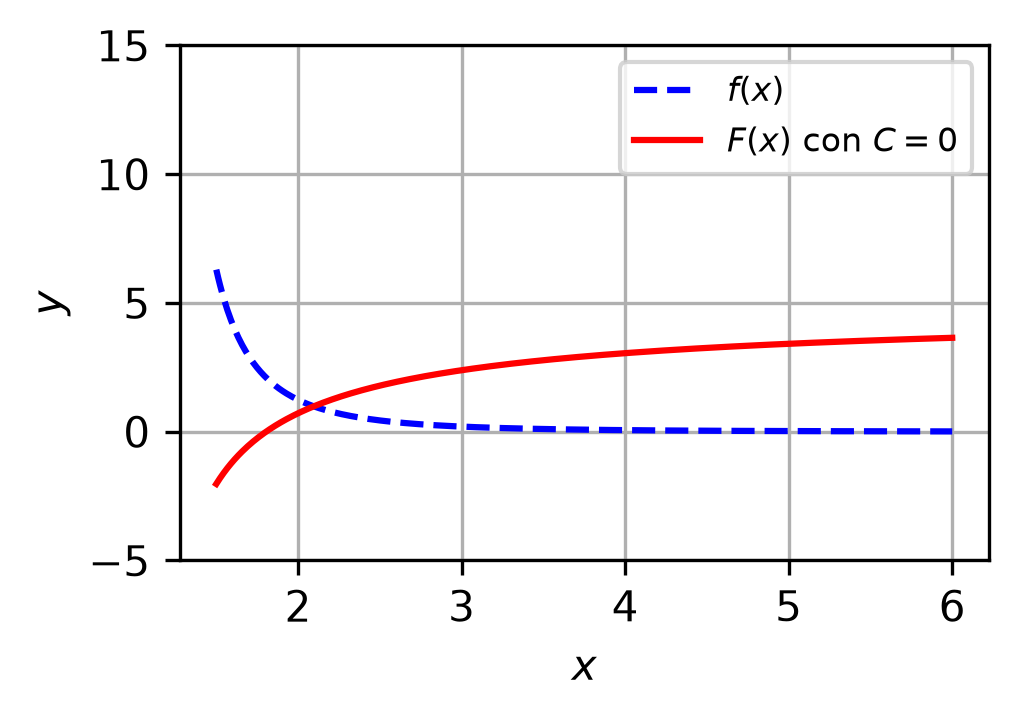
\includegraphics[width=\columnwidth]{semana_03/graficas/SEM03_P23_grafica.png}
	\caption{Representación gráfica de $f(x)$ y su antiderivada $F(x)$ evaluada para la constante de integración $C = 0$ (Problema 23).}
	\label{fig:problema23}
\end{figure}
